\subsection{Getting verbose!}

Although we use colours in SDMs to indicate when an element is to be matched (black), created (green), or destroyed (red), it sometimes makes sense to
indicate these binding operators via explicit stereotypes (i.e., for black-and-white printouts of a model).

\begin{enumerate}
  
\item[$\blacktriangleright$] Open the relevant diagram in the EA editor window and, depending on what type it is, press the \texttt{Verbose} button in
either the \texttt{eMoflon SDM Functions} or \texttt{eMoflon TGG Functions} panel (Fig.~\ref{ea:changeVStatus}).

\vspace{0.5cm}

\begin{figure}[htbp]
\begin{center}
  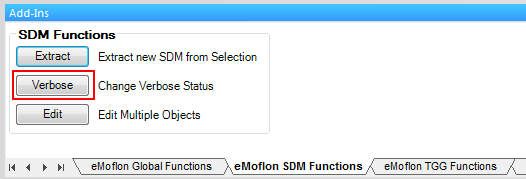
\includegraphics[width=0.8\textwidth]{ea_changeVerboseStatus}
  \caption{Add extra markup to colored links and objects in the current diagram}  
  \label{ea:changeVStatus}
\end{center}
\end{figure}

\item[$\blacktriangleright$] This will add small \texttt{++} or \texttt{-~-} symbols next to deleted and created elements in the current diagram
(Fig.~\ref{ea:verboseSymbols}). Press the button again to deactivate these indicators.

\begin{figure}[htbp]
\begin{center}
  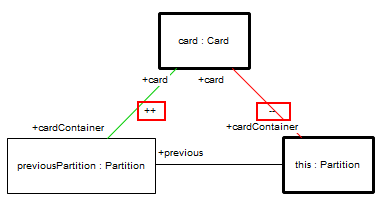
\includegraphics[width=0.7\textwidth]{ea_verboseSymbols}
  \caption{Diagram in verbose mode}  
  \label{ea:verboseSymbols}
\end{center}
\end{figure}

\end{enumerate}
